\documentclass[border=10pt]{standalone}
\usepackage{tikz}
\usepackage{xcolor}

\begin{document}
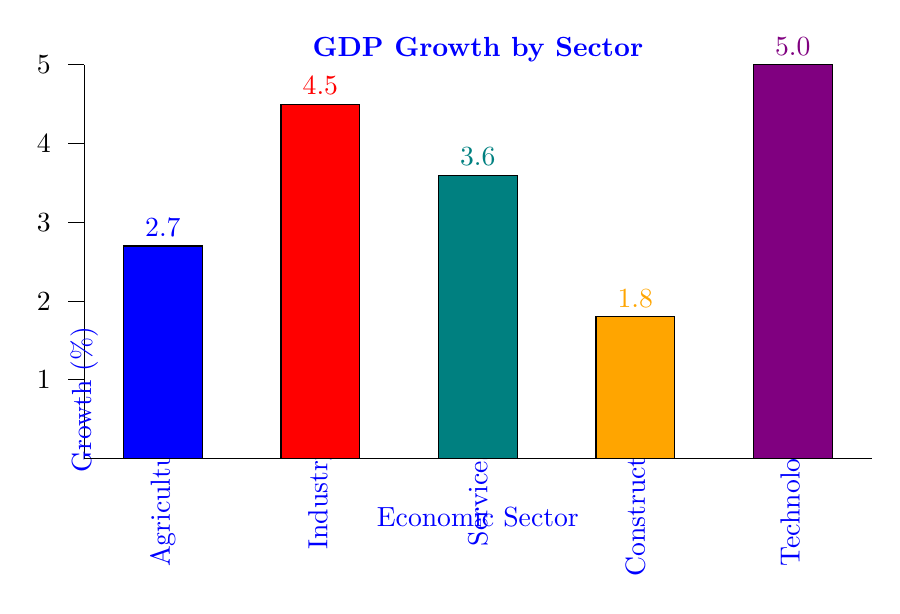
\begin{tikzpicture}
% Define colors
\definecolor{agriculture}{RGB}{0,0,255}
\definecolor{industry}{RGB}{255,0,0}
\definecolor{services}{RGB}{0,128,128}
\definecolor{construction}{RGB}{255,165,0}
\definecolor{technology}{RGB}{128,0,128}

% Title
\node[font=\bfseries, blue] at (5, 5.2) {GDP Growth by Sector};

% Y-axis
\draw (0,0) -- (0,5);
% Y-axis label
\node[blue, rotate=90, left=0.7cm] at (0, 2.5) {Growth (\%)};
% Y-axis ticks and labels
\foreach \y in {1,...,5} {
    \draw (0,\y) -- (-0.2,\y);
    \node[left] at (-0.3,\y) {\y};
}

% X-axis
\draw (0,0) -- (10,0);
% X-axis label
\node[blue, below] at (5, -0.5) {Economic Sector};

% Sector labels (rotated 90 degrees)
\node[blue, rotate=90, anchor=center] at (1,-0.5) {Agriculture};
\node[blue, rotate=90, anchor=center] at (3,-0.5) {Industry};
\node[blue, rotate=90, anchor=center] at (5,-0.5) {Services};
\node[blue, rotate=90, anchor=center] at (7,-0.5) {Construction};
\node[blue, rotate=90, anchor=center] at (9,-0.5) {Technology};

% Bars
\draw[fill=agriculture] (0.5,0) rectangle (1.5,2.7);
\node[agriculture, above] at (1,2.7) {2.7};

\draw[fill=industry] (2.5,0) rectangle (3.5,4.5);
\node[industry, above] at (3,4.5) {4.5};

\draw[fill=services] (4.5,0) rectangle (5.5,3.6);
\node[services, above] at (5,3.6) {3.6};

\draw[fill=construction] (6.5,0) rectangle (7.5,1.8);
\node[construction, above] at (7,1.8) {1.8};

\draw[fill=technology] (8.5,0) rectangle (9.5,5.0);
\node[technology, above] at (9,5.0) {5.0};

\end{tikzpicture}
\end{document}